\documentclass{article}

% ------------------- PACKAGES -------------------
\usepackage[margin=1in]{geometry}   % reasonable margins
\usepackage[mathlines]{lineno}%
\usepackage{
            setspace,   % spacing control
            titlesec,   % formatting section headers
            graphicx,   % for figures if needed
            hyperref,   % for hyperlinks
            parskip,    % spacing between paragraphs
            amsmath, 
            amssymb, 
            mathtools,
            siunitx,
            bm,
            tabularx,
            subcaption,
            % svg
             }
\DeclareGraphicsRule{.tif}{png}{.png}{`convert #1 `basename #1 .tif`.png}
\usepackage[
backend=biber,
]{biblatex}
\addbibresource{bibliography.bib}
% ------------------- FORMATTING -------------------
\setstretch{1.15}                   % line spacing
\titleformat{\section}{\large\bfseries}{\thesection}{1em}{} % section formatting
\titleformat{\subsection}{\normalsize\bfseries}{\thesubsection}{1em}{} % subsection formatting

% ------------------- TITLE INFO -------------------
\title{\vspace{-1cm}Cosmic Ray Flux Reconstruction using Machine Learning}
\author{Carter Chapman, Andrei Gogosha \\ Phys/Astr 448}
\date{\today}
\usepackage{float}
%-------- DOCUMENT -------------------
\begin{document}
\maketitle
\vspace{-0.5cm}

% ------------------- ABSTRACT -------------------

\begin{abstract}


We analyze data from the Pierre Auger Observatory to identify which atmospheric variables most affect cosmic-ray count rates. Using several years of temperature, pressure, and air density measurements, we train a linear \texttt{SGDRegressor} and a nonlinear \texttt{HistGradientBoostingRegressor}, optimized via cross-validation. The \texttt{SGDRegressor} achieves \(\mathbf{7.87 \pm 0.01}\) MAE, while the gradient boosting model improves accuracy to \(\mathbf{6.59 \pm 0.03}\) MAE. SHAP-based feature importance reveals the dominant atmospheric drivers. Our results demonstrate that machine-learning methods, particularly gradient boosting, effectively model the atmospheric modulation of cosmic-ray flux.

\end{abstract}

% ------------------- BACKGROUND AND MOTIVATION -------------------
\section{Introduction}
High-energy particles enter Earth’s atmosphere and interact to produce secondary particles, including high-energy muons and nucleons. Gamma-ray telescopes and particle detectors around the world record these interactions daily. If an experiment is searching for a specific interaction, the flux and nature of these secondary particles must be well understood.
Temperature, pressure, and air density are weather properties known to influence cosmic ray showers \cite{cosmic_climate} and can lead to unexpected variations in measured flux. Machine learning provides an ideal way to study this relationship due to its ability to handle large datasets with many interdependent variables. The boosted model used in this work builds an ensemble of decision trees that iteratively improve upon previous predictions by correcting regions of poor fit. The SGD Regressor is a linear model, making it a useful baseline for comparison against the more complex ensemble methods. Together, these models allow us to evaluate how different learning strategies capture the relationship between atmospheric variables and cosmic ray detection rates.
The Pierre Auger Observatory \cite{auger_website} is a cosmic ray observatory located in Argentina designed to detect high-energy cosmic rays. It does this through two main methods: tracking particle interactions in large water-Cherenkov detectors on the surface and observing ultraviolet radiation from air showers in the upper atmosphere \cite{auger_website}. The observatory provides an open dataset containing 81,121 showers detected via the ultraviolet fluorescence method, along with complementary data from the surface detectors and atmospheric measurements from five meteorological stations in the region. These datasets are available in JSON and CSV formats and include information on particle hits for detectors and weather features such as temperature, pressure, and density. To our knowledge, no published studies have yet used machine learning to predict atmospheric particle flux based on weather variables, although the effects of weather on cosmogenic particles have been explored analytically \cite{LuszczakChan2025}\cite{Maghrabi2023}. Our approach aims to more accurately model cosmic ray flux while incorporating environmental variables that are typically neglected in current analyses \cite{Coleman:2017icrc}.
% \begin{equation}\label{eq:r_flux}
%     S\left(r_{\text{opt}}\right)=S_{0}\left(1+\alpha_{P}\left(P-P_{0} \right) +\alpha_{\rho} \left( \rho_{\text{d}} - \rho_{0}\right) + \beta_{\rho}\left(\tilde{\rho} - \rho_{\text{d}} \right)\right)
% \end{equation}

% ------------------- METHODS -------------------
\section{Methods}
\subsection{Data preprocessing}

The Pierre Auger Open Release data \cite{auger_data} provides the data for this search. The scaler data contains 15-minute averaged particle event rates uncorrected for atmospheric pressure dependence, fraction of the array in operation, and Unix timestamps. The atmospheric data contains temperature, barometric pressure, humidity-corrected air density, and Unix timestamps taken every five or ten minutes with gaps of ten minutes to three hours interpolated from the endpoints of the interval. If the gap was longer than three hours, the period was not included. To account for the differing rates of atmospheric data, cosmic ray data, and missing periods of atmospheric data, we time-aligned the scaler and atmospheric data using timestamps. Due to changes made in the Pierre Auger Data Taking strategy, there are two distinct populations in the count rate distributions shown below \ref{fig:Count_Rate}. 

\begin{figure}[!ht]
  \centering
  \includegraphics[width=0.5\textwidth]{plots/YearvsRate.png}
  \caption{Particle Count Rate by Year}
  \label{fig:Count_Rate}
\end{figure}

The two populations come from years after 2011 and years before 2010. The exact reason for this is unclear; however, changes made to the trigger scheme \cite{PierreAuger2011Scaler} in the past offer a likely explanation for this behavior. For this reason, all our models used only data that came after 2012. This also led us to use the 'year' as a one-hot encoded feature using the \texttt{OneHotEncoder} preprocessor from \texttt{scikit-learn}. 

The final list of features used for training our models is: Temperature, Pressure, Air Density, Array Fraction, Density 2 Hours Prior, and \texttt{OneHotEncoder} Year. 

\subsection{Machine Learning Models}
All trained models used a nested cross-validation scheme of five outer and three inner shuffled folds when performing hyperparameter optimization. The mean absolute error (MAE) was used as the scoring metric for training and performance evaluation.

\subsubsection{SGDRegressor}
For modeling the linear relationship between atmospheric conditions and cosmic-ray flux, we trained an \texttt{SGDRegressor} from \texttt{scikit-learn} \cite{scikit-learn}. 
Hyperparameter optimization was performed on which loss function the regressor optimizes, the regularization term \texttt{penalty} and its weighting factor \texttt{alpha}, the elastic net mixing parameter \texttt{l1\_ratio}, and the threshold value where the Huber loss changes from quadratic to linear \texttt{epsilon}. When training data was scaled using the \texttt{StandardScaler} function from \texttt{scikit-learn}.
The hyperparameter values optimized are summarized in Table \ref{tab:sgd_hyperparam}

\begin{table}[!ht]
\centering
\caption{Hyperparameter values optimized for the \texttt{SGDRegressor}.}
\label{tab:sgd_hyperparam}
\begin{tabular}{| l|l l l l l|}
\hline
\texttt{loss}     & squared\_error & huber & & & \\\hline
\texttt{penalty}  & l1 & l2 & elasticnet & None & \\\hline
\texttt{alpha}    & 0.00001 & 0.0001 & 0.001 & & \\\hline
\texttt{l1\_ratio} & 0.1 & 0.5 & 1 & & \\\hline
\texttt{epsilon}  & 0.1 & 0.5 & 1 & 5 & \\\hline
\end{tabular}
\end{table}


\subsubsection{HistGradientBoostingRegressor}

For modeling the non-linear relationships between atmospheric conditions and cosmic-ray flux, we trained a \texttt{HistGradientBoostingRegressor } Decision Tree from \texttt{scikit-learn} \cite{scikit-learn}. 
We explored a grid of hyperparameters as summarized in Table~\ref{tab:hgb_hyperparam}. The maximum tree depth (\texttt{max\_depth}) controls the complexity of each individual tree, while the number of boosting iterations (\texttt{max\_iter}) determines how many trees are sequentially added to the ensemble. The learning rate (\texttt{learning\_rate}) scales the contribution of each tree, and the loss function (\texttt{loss}) specifies whether the model minimizes squared error or absolute error. Finally, the minimum number of samples per leaf (\texttt{min\_samples\_leaf}) sets the smallest number of training examples required to form a leaf, helping to prevent overfitting.



\begin{table}[!ht]
\centering
\caption{Hyperparameter values optimized for the \texttt{HistGradientBoostingRegressor}.}
\label{tab:hgb_hyperparam}
\begin{tabular}{| l|l l l l|}
\hline
\texttt{max\_depth}       & 3  & 6  & 10 & None \\\hline
\texttt{max\_iter}        & 50 & 100 & &  \\\hline
\texttt{learning\_rate}   & 0.05 & 0.1 & &  \\\hline
\texttt{loss}             & squared\_error & absolute\_error & &  \\\hline
\texttt{min\_samples\_leaf} & 5 & 10 & 15 &  \\\hline
\end{tabular}
\end{table}

\subsection{SHAP Feature Importance}

To interpret the contributions of individual atmospheric variables to the predicted cosmic-ray count rates, we used SHapley Additive exPlanations (SHAP) \cite{NIPS2017_8a20a862}. SHAP is a model-agnostic framework that assigns each feature an importance value for a particular prediction, based on cooperative game theory. For the \texttt{HistGradientBoostingRegressor}, we computed SHAP values using the TreeExplainer\cite{lundberg2020local2global}, which leverages the structure of gradient-boosted trees for an efficient and exact computation. For the \texttt{SGDRegressor}, which is a linear model, we used LinearExplainer, which computes SHAP values analytically based on the model coefficients, allowing us to directly assess the contribution of each feature to the predicted count rate. For each feature, we examined both the mean absolute SHAP value across the test set, which quantifies overall importance, and the distribution of SHAP values, which reveals whether higher or lower feature values increase the predicted count rate. This analysis allowed us to identify which atmospheric variables, such as air pressure, temperature, or density, modulate the predicted particle flux the most, providing information on the physical drivers of the observed variations.

\section{Results}
Since the performance of both the \texttt{SGDRegressor} and \texttt{HistGradientBoostingRegressor} models with only the atmospheric data showed worse performance than with the \texttt{OneHotEncoder} year feature analogous plots to those found in Figure \ref{fig:sgd_plots_onehot} and Figure \ref{fig:hgb_pred_vs_act_onehot} and \label{fig:hgb_pred_vs_act_onehot_hist} have been omitted for brevity, but can be found in the training notebooks \cite{Gogosha_UNC-MLPhysAstr_Final_Project}. 
\subsection{SGDRegressor}


% \subsubsection{Atmospheric Data Features}
When using temperature, pressure, air density, density 2 hours before, and array fraction as our training features, the \texttt{SGDRegressor} model achieved an MAE of \( 10.88 \pm 0.01868\) and \( 7.8748 \pm 0.01025\) when including the \texttt{OneHotEncoder} year feature. The hyperparameters that perform the best are in Table \ref{tab:sgd_hyperparam_final}.
\begin{table}[!ht]
\centering
\caption{Best Performing Hyperparameter values for the \texttt{SGDRegressor} model.}
\label{tab:sgd_hyperparam_final}
\begin{tabular}{|l | l | l| }
\hline
                   & Atmospheric Data & \texttt{OneHotEncoder} Year  \\\hline
\texttt{loss}      & huber      & huber \\
\texttt{penalty}   & elasticnet & l1 \\
\texttt{alpha}     & 0.0001     & 0.0001 \\
\texttt{l1\_ratio} & 0.5        & 0.1 \\
\texttt{epsilon}   & 1          & 1  \\\hline
\end{tabular}
\end{table}
The results for the model trained with \texttt{OneHotEncoded} features are in Fig \ref{fig:sgd_plots_onehot}.

\begin{figure}[!ht]
%use \ref{} ro reference plot somewhere
  \centering
  \begin{subfigure}[b]{0.31\linewidth}
    \includegraphics[width=\linewidth]{plots/pred_vs_act_onehot.png}
    \caption{Predicted vs Actual Cosmic Ray Flux grouped by Year}
    \label{fig:sgd_pred_vs_act_onehot}
  \end{subfigure}
  \begin{subfigure}[b]{0.31\linewidth}
    \includegraphics[width=\linewidth]{./plots/shap_onehot_bar.png}
    \caption{\(\text{mean}\left(\lvert \text{SHAP}\rvert \right) \) value for each feature}
    \label{fig:sgd_shap_bar_onehot}
  \end{subfigure}
  \begin{subfigure}[b]{0.31\linewidth}
    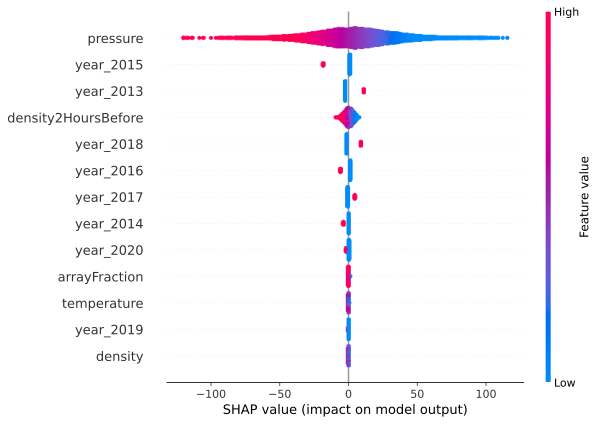
\includegraphics[width=\linewidth]{./plots/shap_onehot_beeswarm.png}
    \caption{Each instance features SHAP values. The points' color gives the feature value, the x-axis represents the impact it had on the model, and the width of the distribution represents the density of points at that SHAP value.}
    \label{fig:sgd_shap_bee_onehot}
  \end{subfigure}
  \caption{\texttt{OneHotEncoder} Year Feature Performance and Feature Importance plots}
  \label{fig:sgd_plots_onehot}
\end{figure}

Plot (\ref{fig:sgd_pred_vs_act_onehot}) shows the models' predicted vs actual values. 
The data points are also colored by year to provide more insight into problematic years. An \(R^{2}\) value of \(0.883\) means that the model accounts for most of the variance in the data, but still has some large outliers unexplained by the model. As you can see in plot (\ref{fig:sgd_pred_vs_act_onehot}), 2016 has some large outliers which are likely the largest contributors to the bias in our model. This suggests that either our features are not providing enough information for our model to fully capture the relationship between our features or the relationship between our features is nonlinear. The results in section \ref{hgb_results} suggest that the relationship is non-linear due to the better performance of the \texttt{HistGradientBoostingRegressor} model. Plot (\ref{fig:sgd_shap_bar_onehot}) gives the average SHAP value for each of the features. It shows that pressure contributes the most to the model's output; on average, it changes the predicted count rate by \(20\,\dfrac{counts}{s}\). This plot also shows that, contrary to our proposal's expectation, density is not the most important feature; it is the least important. Plot (\ref{fig:sgd_shap_bee_onehot}) shows the distribution of SHAP values by feature, and provides more insight into the maximum and minimum impact features have on the predictions.


\subsection{HistGradientBoostingRegressor}\label{hgb_results}

When using temperature, pressure, air density, density 2 hours before, and array fraction as our training features, the \texttt{HistGradientBoostingRegressor} model achieved an MAE of 
\( 10.1793 \pm 0.02920\) and an MAE of \( 6.5860 \pm 0.02472\) when including year as a feature. The hyperparameters that perform the best are in Table \ref{tab:hgb_onehot_hyperparam_final}
\begin{table}[!ht]
\centering
\caption{Best Performing Hyperparameter values for the \texttt{HistGradientBoostingRegressor} model.}
\label{tab:hgb_onehot_hyperparam_final}
\begin{tabular}{| l | l | l |}
\hline
& Atmospheric Data & \texttt{OneHotEncoder} Year  \\\hline
\texttt{max\_depth} &   None    & None      \\
\texttt{max\_iter} &  100  & 100 \\
\texttt{learning rate} &   0.1   & 0.01     \\
\texttt{loss} & absolute\_error  & squared\_error        \\
\texttt{min\_samples\_leaf} & 10   & 10          \\\hline
\end{tabular}
\end{table}

The results with the \texttt{OneHotEncoded} features and the boosting method are given below \ref{fig:hgb_pred_vs_act_onehot}


\begin{figure}[!ht]
  \centering
  \begin{subfigure}[b]{0.31\linewidth}
    \includegraphics[width=\linewidth]{plots/hgd_pred_vs_act_onehot_hist.png}
    \caption{Predicted vs Actual Cosmic Ray Flux grouped by Year}
    \label{fig:hgb_onehot_preds_vs_act_hist}
  \end{subfigure}
  \begin{subfigure}[b]{0.31\linewidth}
    \includegraphics[width=\linewidth]{./plots/shap_onehot_bar_hist.png}
    \caption{Average absolute SHAP value for each of the five atmospheric features}
    \label{fig:hgb_onehot_shap_bar}
  \end{subfigure}
  \begin{subfigure}[b]{0.31\linewidth}
    \includegraphics[width=\linewidth]{./plots/hgd_shap_onehot_beeswarm_hist.png}
    \caption{Each instance features SHAP values. The points' color gives the feature value, the x-axis represents the impact it had on the model, and the width of the distribution represents the density of points at that SHAP value.}
    \label{fig:hgb_onehot_shap_bee}
  \end{subfigure}
  \caption{OneHotEncoded Feature Performance and Feature Importance plots}
  \label{fig:hgb_pred_vs_act_onehot}
\end{figure}


Plot \ref{fig:hgb_onehot_preds_vs_act_hist} shows the models' predicted vs actual values. Compared to \ref{fig:sgd_pred_vs_act_onehot}, the boosted model is able to capture non-linear relationships for problematic years such as 2015, and 2016. Other years that still remain difficult for the model to train is 2019. This could come from a change in a triggering scheme or an increase in cosmic rays due to other physics processes. An $R^2$ value of 0.923 means the model accounts for the vast majority of the variance in the data. Plot (\ref{fig:hgb_onehot_shap_bar}) gives the average SHAP value for each of the features. It confirms that pressure is the most important feature by a wide margin, as the pressure value on average changes the predicted count rate by \(21\,\dfrac{counts}{s}\). It is also shown that the year is the second most important feature behind pressure. Density also plays a much more significant role for the boosted model than it does for \texttt{SGDRegressor}. Plot (\ref{fig:hgb_onehot_shap_bee}) shows how the boosted model treats the \texttt{OneHotEncoded} Year features differently as the SHAP values have larger ranges of impact on the count rate.



\section{Conclusion}

Both the \texttt{SGDRegressor} and the \texttt{HistGradientBoostingRegressor} accurately predict particle flux from atmospheric data, with the boosted model achieving superior performance due to its ability to capture non-linear relationships. It also trains more efficiently, reaching better accuracy in significantly less time. Initial exploration suggested that the year of data collection influenced the model, a result confirmed through SHAP analysis \cite{NIPS2017_8a20a862}. SHAP further identified pressure as the most impactful feature in predicting flux variations, counter to our proposed hypothesis of density being the most important feature. These results demonstrate that machine-learning methods can effectively characterize atmospheric modulation of cosmic-ray flux. Future work should extend these techniques to broader geographic settings and explore their potential for predicting additional cosmic-ray properties, such as energy distributions or particle interactions.

A GitHub repository containing our training notebooks, data, preprocessing scripts, and documentation is available in the references \cite{Gogosha_UNC-MLPhysAstr_Final_Project}.

\printbibliography
\end{document}

